\clearpage
\chapter{Machine Learning}\label{sec:machinelearning}

ROIs are artificial regions created by the CMSSW mechanism, which are displaced vertex candiates.
ROIs contain thorough information about fitted tracks, vertices, and isolation information, after following the formation procedure described in the previous section. 
The exhaustive variables saved in each ROI contain information, which directly and indirectly tells whether the ROI is from signal process or background process.
Given the extensive amount of variables within ROIs, it's inappropriate to use ROIs' single or a few variabes as our tagging variables, like in ZH analysis ~\cite{ZHAN}.  
It is also ineffcient to implement a cut-based approach due to having approximately 20-30 variables from ROI.
Optimization process for all 20-30 variables would be extremley time-consuming, inefficient, and error-prone as well.
Therefore, the analysis exploits machine learning (ML) for these multivariate analysis.
Boosted decision trees will also face similar problem as cut-based analysis, although to a lesser extent.
Deep Neural Network are the most adaptable ML algorithm for this analysis method, in which the analysis inputs extensive list of ROI variables into a neural network, and receives a final score to discriminate ROIs that arise in signal process versus background processes. 

  
\section{Machine Leaning Software}\label{sec:MLSW}

The analysis uses Keras-Tensorflow via CMSSW.
CMSSW includes Keras-Tensorflow, which enables simple and easy usage of keras-Tensorflow with simple cmsenv command in various CMS remote clusters. 
For CMSSW\_10\_6\_12 (to have access for BPH trigger path), Keras-Tensorflow version is 2.3.1.
It runs with CPUs and GPUs.
CMSSW includes image container for Keras-Tensorflow and researchers can submit remote batch jobs for its ML training.
The analysis tested multiple variables (such as epoch numbers, batch sizes, phi sizes, f sizes) of our DNN layers thanks to submission of remote batch jobs with CMSSW's Keras-Tensorflow image container.
Subsection ~\ref{sec:Ethan} below details the numerical results from such tests.
The analysis also tested different combinations of signal vs background datasets for maximum discriminant power. 
The list of mass scale and lifetime tested for signal points are listed in subsection~\ref{sec:Ethan2}. Different SM physics process (and their compositions) tested for background process are also listed in subsection~\ref{sec:Ethan2}
The analysis used the tensorflow protocol buffer files, which were trained with parameters and physics process as in Table~\ref{tab:ROIParam}. 

\begin{table}[htb]
\caption{Tensorflow information}
\begin{center}
\begin{tabular}{r|l}\hline
Epoch & 300 \\
batch size & 250 \\
Phi sizes & ((64,128,256),(32,64,128)) \\
f sizes & (256,128,32) \\
Signal & ggHSSTo4Tau-MS15GeV-c$\tau$100mm  \\
Background & QCD\_Pt120-170\_MuEneriched and TTJets \\
 \hline
 \hline
\end{tabular}
\label{tab:ROIParam}
\end{center}
\end{table}


\section{Machine Learning Input Variable}\label{sec:MLIV}
The extensive variables for input of our DNN are described and categorized in Tables ~\ref{tab:ROITCvars}, ~\ref{tab:ROIANvars}, and ~\ref{tab:ROIEVvars}.

\begin{table}[htb]
\caption{ROI (trackCluster) variables by category}
\begin{center}
\begin{tabular}{r|l|l}\hline
 TrackCluster & Position & TrackClusters.vx() - primaryVertex.X() \\
              & Position & TrackClusters.vy() - primaryVertex.Y() \\
              & Position & TrackClusters.vz() - primaryVertex.Z() \\
              & Covariance & TrackClusters.vertexCovariance()(0,0) \\
              & Covariance & TrackClusters.vertexCovariance()(0,1) \\
              & Covariance & TrackClusters.vertexCovariance()(0,2) \\
              & Covariance & TrackClusters.vertexCovariance()(1,0) \\
              & Covariance & TrackClusters.vertexCovariance()(1,1) \\
              & Covariance & TrackClusters.vertexCovariance()(1,2) \\
              & Track0,1 & Track0,1.pt \\
              & Track0,1 & Track0,1.eta \\
              & Track0,1 & Track0,1.phi \\
              & Track0,1 & Track0,1.dxy \\
              & Track0,1 & Track0,1.dz \\
              & Track0,1 & Track0,1.normalizedChi2 \\
              & Track0,1 & Track0,1.HighPurityInt \\
 \hline
 \hline
\end{tabular}
\label{tab:ROITCvars}
\end{center}
\end{table}


\begin{table}[htb]
\caption{ROI (Annulus) variables by category}
\begin{center}
\begin{tabular}{r|l|l}\hline
 Annulus      & pfCandidate/LostTracks & pfCandidate/LostTracks.pt \\
              & pfCandidate/LostTracks & pfCandidate/LostTracks.eta \\
              & pfCandidate/LostTracks & pfCandidate/LostTracks.phi \\
              & pfCandidate/LostTracks & pfCandidate/LostTracks.dxy \\
              & pfCandidate/LostTracks & pfCandidate/LostTracks.dz \\
              & pfCandidate/LostTracks & pfCandidate/LostTracks.normalizedChi2 \\
              & pfCandidate/LostTracks & pfCandidate/LostTracks.HighPurityInt \\
              & pfCandidate/LostTracks & pfCandidate/LostTracks.DeltaR(trackMomentum) \\
 \hline
 \hline
\end{tabular}
\label{tab:ROIANvars}
\end{center}
\end{table}


\begin{table}[htb]
\caption{Event variables by category}
\begin{center}
\begin{tabular}{r|l|l}\hline
  ROI    & Position & x \\
         & Position & y \\
         & Position & z \\
 \hline
 \hline
\end{tabular}
\label{tab:ROIEVvars}
\end{center}
\end{table}


\begin{figure}[h!]
  \caption{asdasdasd}
  \label{fig:TensorFlow scores}
  \centering
  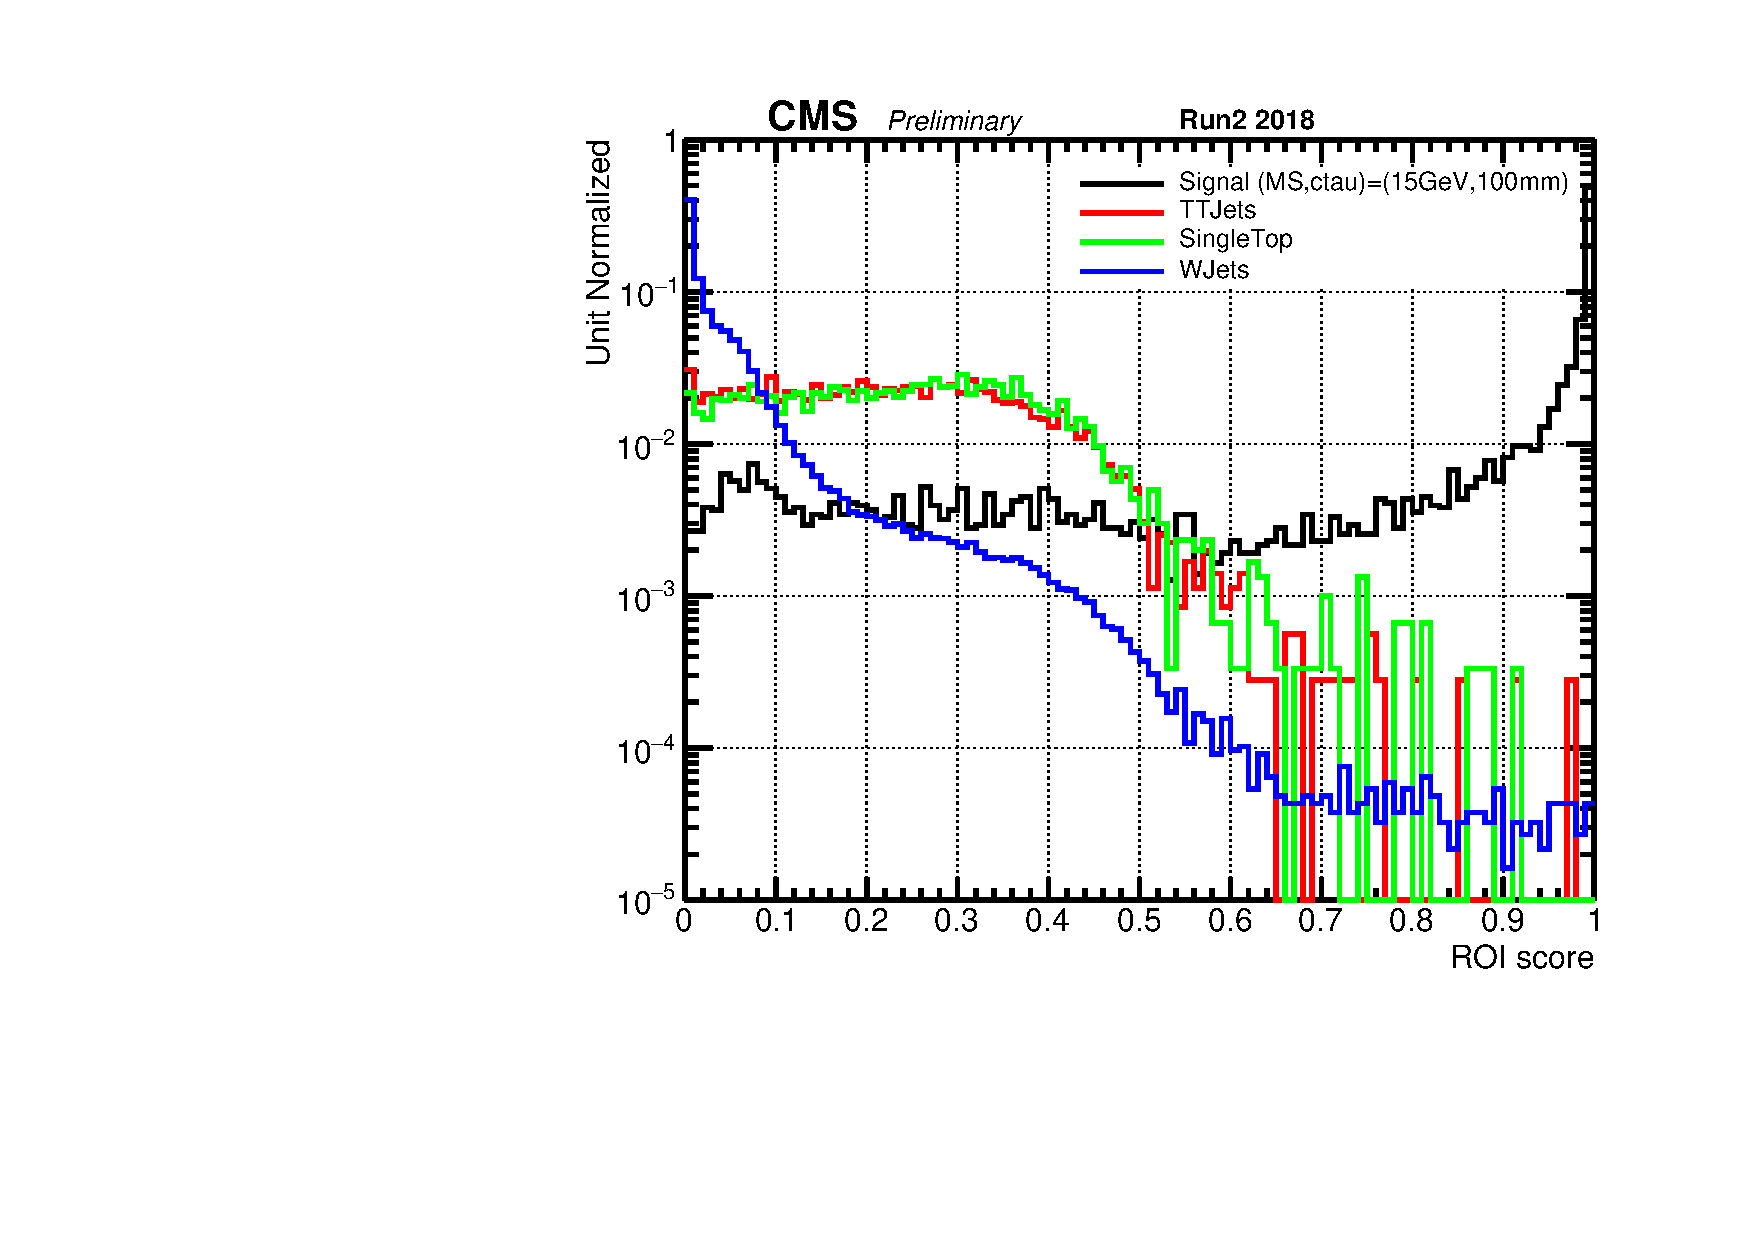
\includegraphics[width=0.67\linewidth]{figs/Tensorflow_Disc_mostrecent.pdf}

\end{figure}

\begin{figure}[h!]
  \caption{Data/MC agreement for ROI scores}
  \label{fig:DataMCscore}
  \centering
  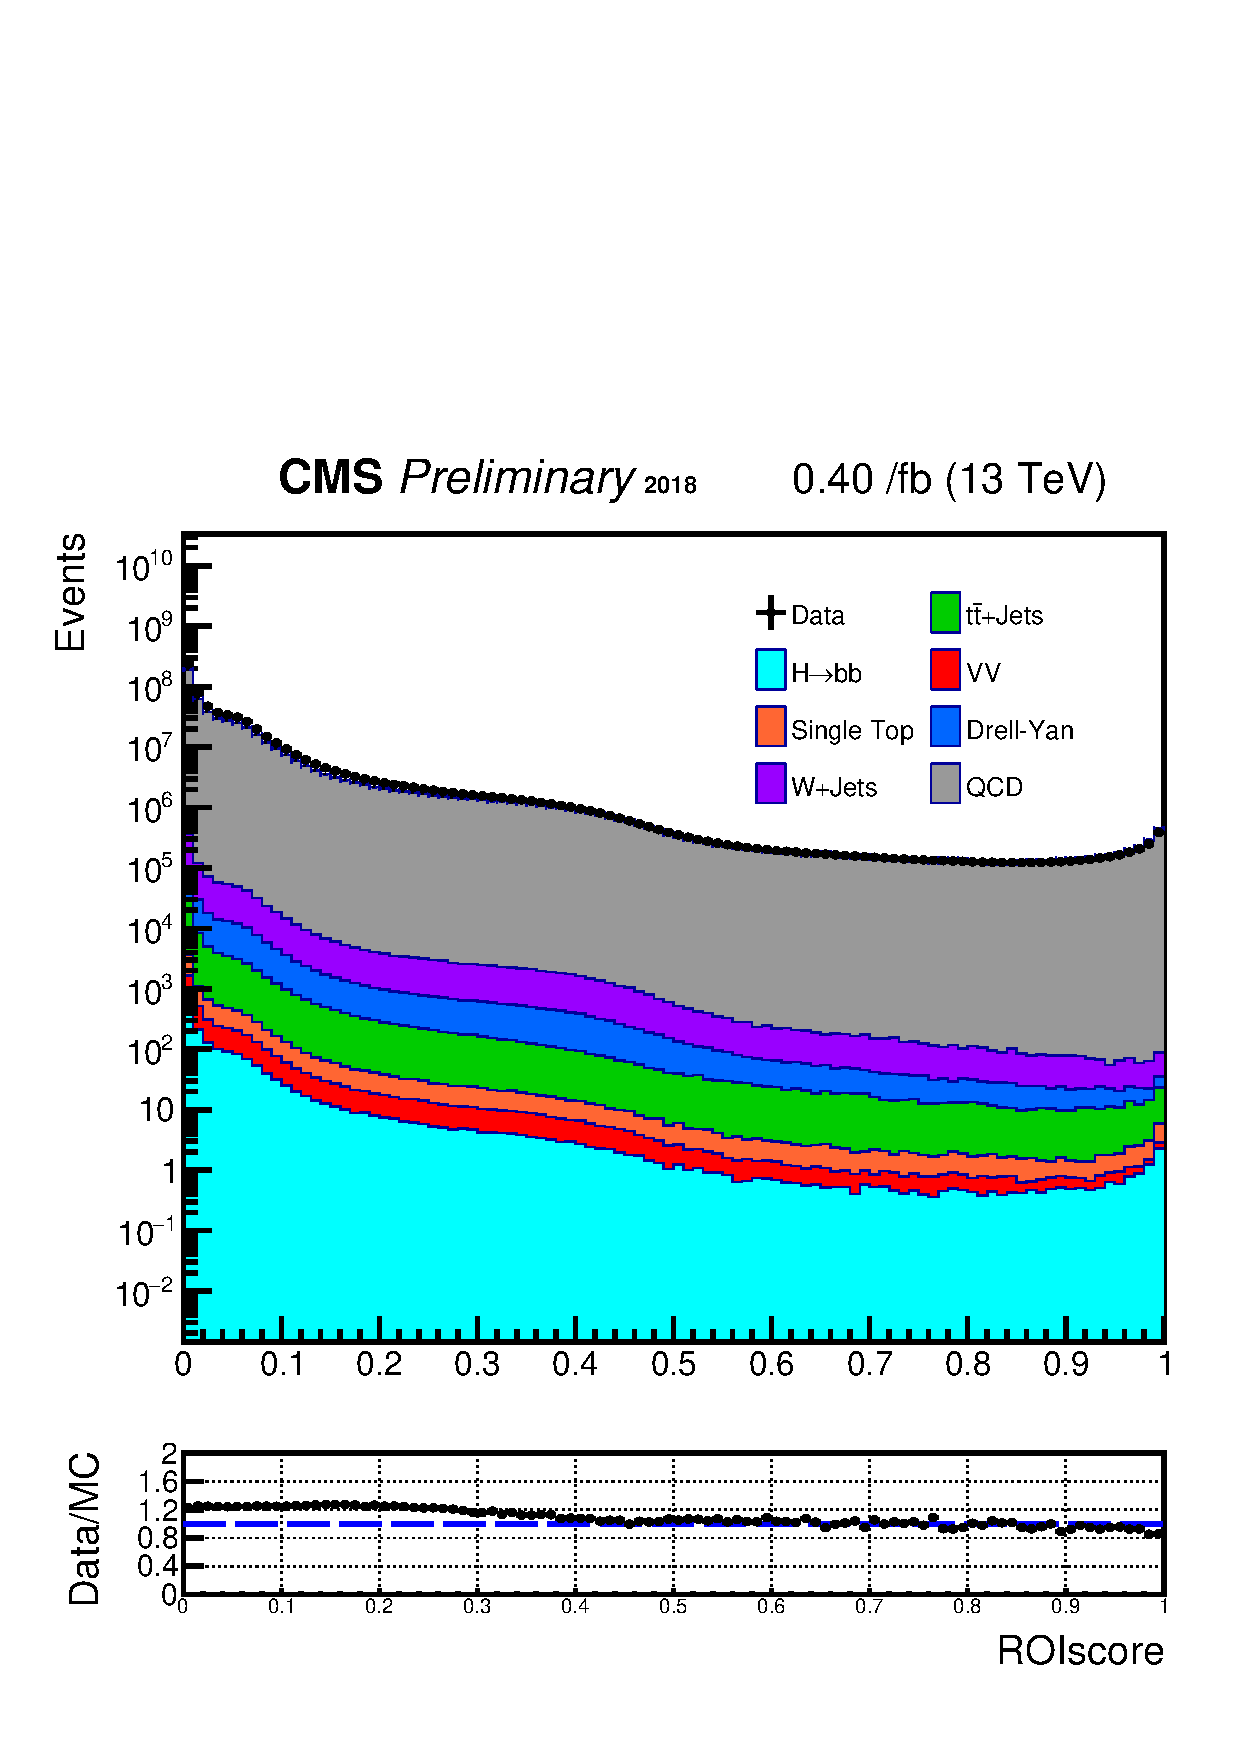
\includegraphics[width=0.67\linewidth]{figs/Data_AnalysisNoteplot_MS-15_ctauS-10_ROIscore.pdf}

\end{figure}


\begin{figure}[h!]
  \caption{Data/MC agreement for loglead/sublead scroes}
  \label{fig:DataMCscore}
  \centering
  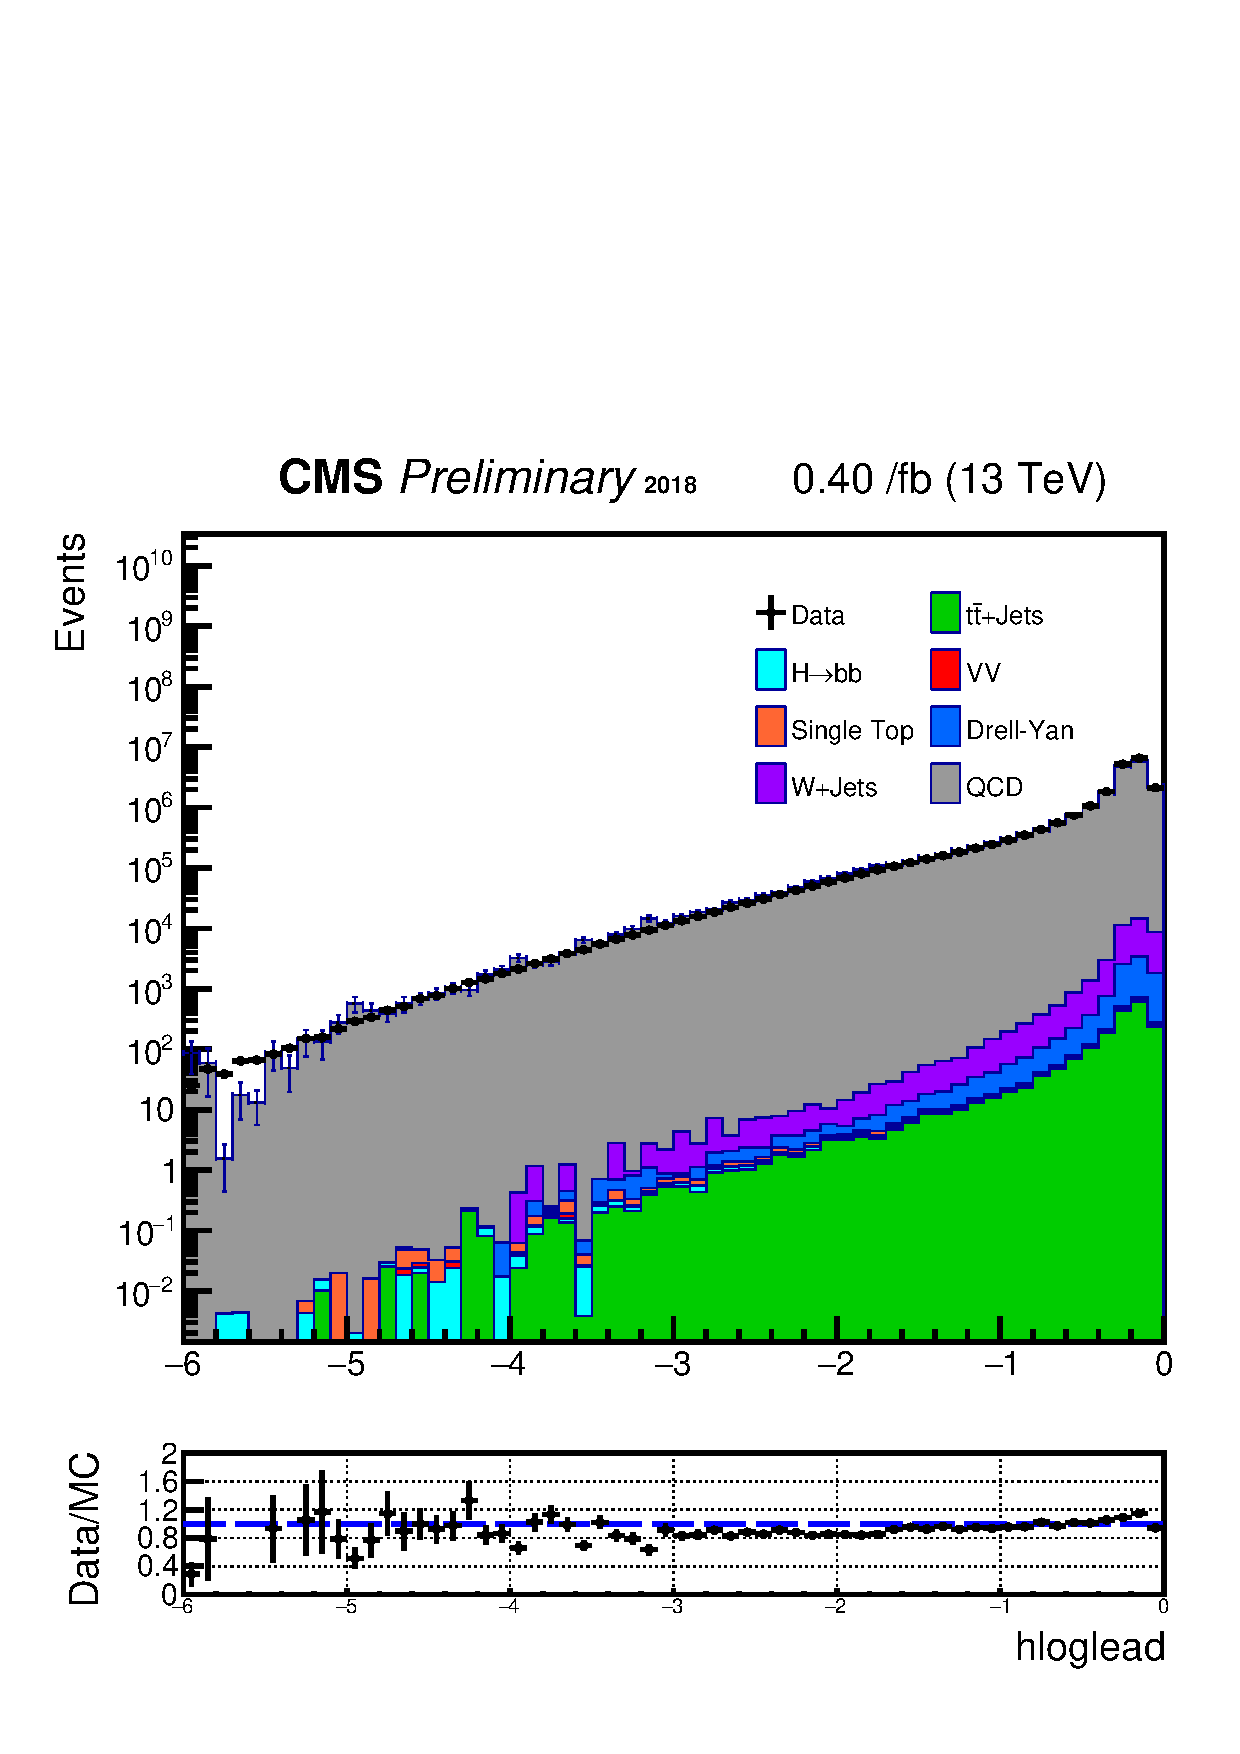
\includegraphics[width=0.47\linewidth]{figs/Data_AnalysisNoteplot_MS-15_ctauS-10_hloglead.pdf}
  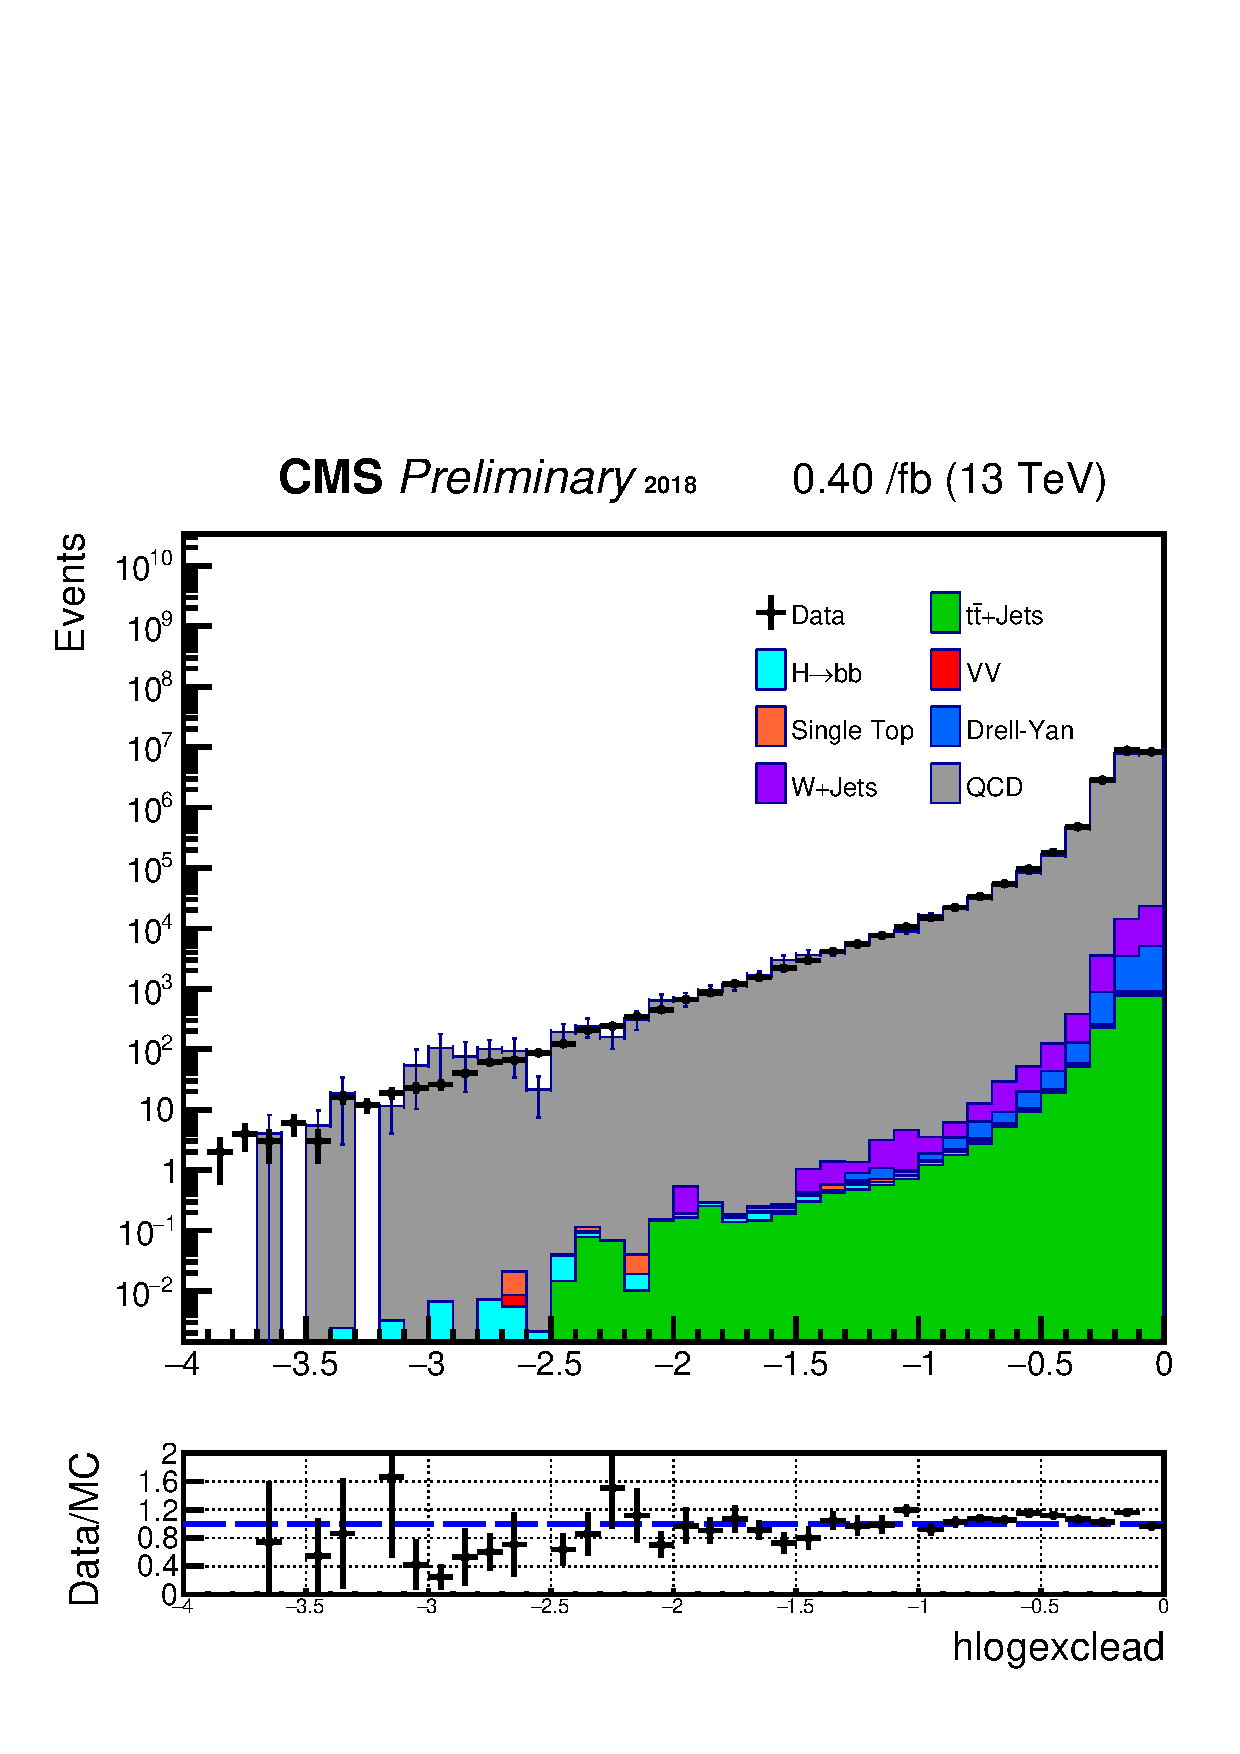
\includegraphics[width=0.47\linewidth]{figs/Data_AnalysisNoteplot_MS-15_ctauS-10_hlogexclead.pdf}
\end{figure}



\section{DNN Variable Test}\label{sec:Ethan}
For Ethan.

\section{Signal and Background MC Test}\label{sec:Ethan2}
For Ethan.

\section{SHAP values}
For Ethan.

